\capitulo{1}{Introducción}


Hoy en día la tecnología está presente en todas nuestras actividades, incluyendo las actividades de ocio como las visitas a los museos. En este trabajo se propone una alternativa a las visitas guiadas dentro del museo. Para generar una mejor experiencia en la visita, el usuario podrá compartir el vídeo capturado por su cámara permitiéndole, además, ver el texto y el vídeo que el guía puede añadir para explicar conceptos. El guía y el visitante además tienen conexión de audio en directo, lo que permite una interacción individualizada o grupal por parte del guía.

Las alternativas de este proyecto son las visitas convencionales, presentadas a continuación:
\begin{itemize}
    \item \underline{Folleto}: Hoja de papel que presenta la información mediante texto o imágenes. La información es muy limitada y si se quiere profundizar en conceptos, no es posible con este medio.
    \item \underline{Audio-guía}: Presenta la información mediante audios, normalmente acompañados de una ruta concreta y organizados mediante salas. La información es limitada, y si se quiere profundizar no es posible.
    \item \underline{Guía presencial}: La información la expone un guía presencial que acompaña a un grupo de visitantes. A veces puede haber problemas de comprensión entre el guía y el usuario, si el grupo es muy grande o la sala está muy llena, además el guía está limitado a la hora de expresarse, a nivel verbal y gesticular.
\end{itemize}

Este proyecto propone nuevas formas de comunicación remota entre usuario y guía, permitiendo que el guía se exprese mediante diversos medios para dar la visita:
\begin{itemize}
    \item \textbf{Verbal}: El guía puede comunicarse vía audio con los usuarios.
    \item \textbf{Escrita}: El guía puede escribir información encima de las obras de arte que estén visualizando los usuarios.
    \item \textbf{Dibujos}: El guía puede dibujar encima de las obras de arte mediante realidad virtual, en caso que se necesite.
\end{itemize}

En la figura 1.1 se puede observar la interfaz del guía dibujando encima de una obra de arte. Una vez guardado el dibujo, los usuarios lo podrán visualizar si enfocan a esa obra de arte con la cámara de vídeo de su dispositivo.
\FloatBarrier
\begin{figure}[h]
    \centering
    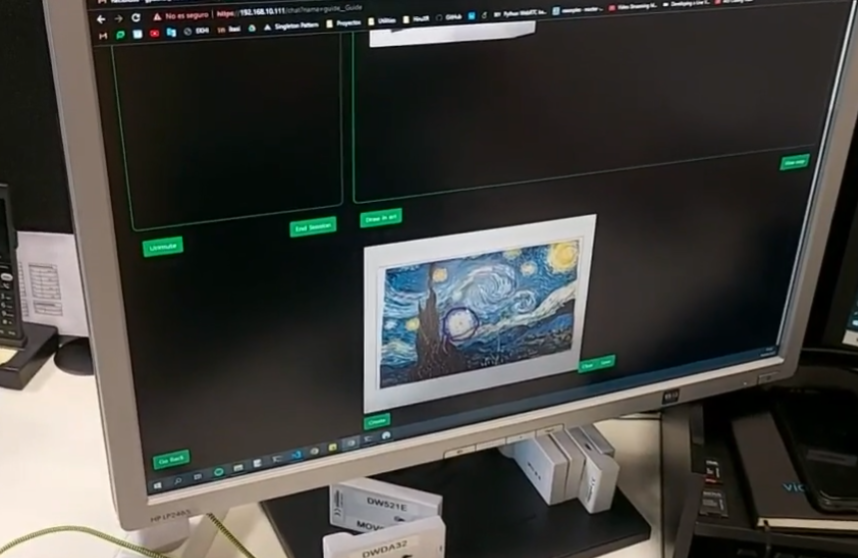
\includegraphics[width=10cm,height=10cm,keepaspectratio]{img/guide drawing.png}
    \caption{Interfaz del guía. Se puede observar la imagen de una obra de arte sobre la que el guía puede dibujar.}
    \label{fig:exmaple_guide drawing}
\end{figure}
\FloatBarrier
Esto puede generar más comprensión por parte del usuario sobre los conceptos explicados, además de poder hacerlo de manera remota sin necesidad de estar allí de manera presencial.


En esta solución se implementa la tecnología \textit{Ultra Wide Band (UWB)} como alternativa a la tecnología \textit{GPS}, debido a que \textit{GPS} no es un sistema de localización fiable dentro de edificios. La localización dentro de edificios (localización \textit{indoor}) se quiere realizar debido a que los usuarios se mueven entre salas. Esto permite hacer \textit{geofencing} y que un usuario pueda ver un mensaje de bienvenida la primera vez que entra a una sala.

Respecto a \textit{UWB}, es similar a la tecnología comunicación muy extendida \textit{Bluetooth Low Energy (BLE)}, pero con mejores prestaciones, para intentar que el sistema sea lo menos propenso a errores y así el cálculo de la localización de los usuarios sea lo más precisa posible. 

En al figura 1.2 aparece representado un sistema típico de interconexión \textit{UWB} para la ubicación de un visitante. En la figura se han utilizado los siguientes términos:
\begin{figure}[t]
    \centering
    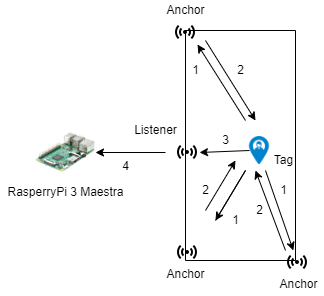
\includegraphics[width=10cm,height=10cm,keepaspectratio]{img/Esquema Conexiones UWB.drawio.png}
    \caption{Disposición de placas \textit{UWB} para la localización \textit{indoor}.}
    \label{fig:exmaple_UWB}
\end{figure}

\begin{itemize}
    \item \textbf{Anchor}: rol que ejerce una placa \textit{UWB} ubicada físicamente en los límites de una sala del museo y que se mantiene estática y pasiva para que otras placas puedan consultar su posición en el proceso de cálculo de la localización.
    \item \textbf{Tag}: rol que ejerce una placa \textit{UWB} transportada por el visitante del museo. Es la encargada de realizar su propia triangulación consultando, en el proceso, la posición de las placas \textit{Anchor}. Una vez calculada su posición se la envía a la placa \textit{Listener} para su gestión.

    \item \textbf{Listener}: rol que ejerce una placa \textit{UWB} encargada de recoger todas las posiciones de las placas Tag y enviárselas a la \textit{Raspberry}.
    \item \textbf{Raspberries Pi 3}: es un ordenador integrado en una placa. Es referenciado como \textit{raspberry}, siendo el intermediario entre la red de placas \textit{UWB} y la \textit{API}, diseñada para la comunicación entre las interfaces de guía y usuario.
\end{itemize}


Una vez se tiene la posición de los usuarios, la idea es representarlo en un mapa a través de una aplicación web o \textit{webapp}, así el guía que esté dando una visita en el museo tendrá más información y contexto del sitio exacto del grupo visitante.

\begin{figure}[t]
    \centering
    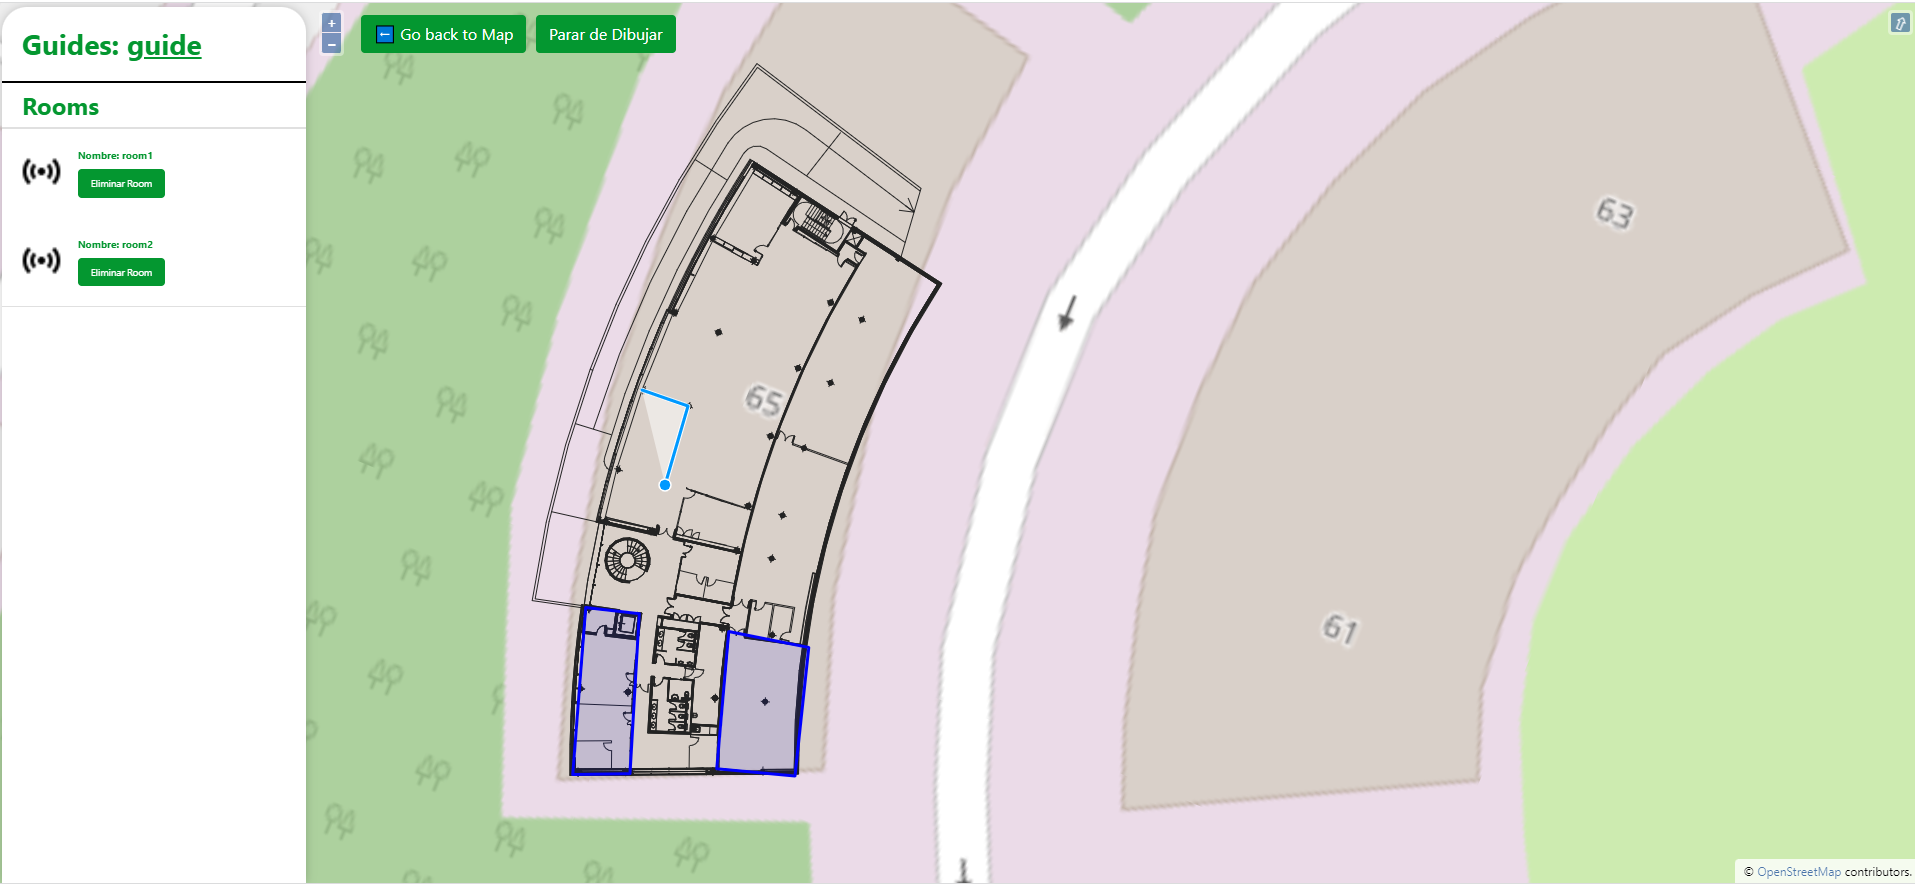
\includegraphics[width=10cm,height=10cm,keepaspectratio]{img/EditRoom.png}
    \caption{Imagen del sistema de dibujado de las salas (en azul). A la izquierda aparece un sidebar con el nombre de todas las salas (rooms) activas.}
    \label{fig:exmaple_room_editing}
\end{figure}

Teniendo la localización en el mapa de los usuarios, el guía podrá crear salas en un mapa dibujándolas, que llamaremos \textit{\textbf{Rooms}}, además contará con un \textit{sidebar} que lista todas las \textit{Rooms} que existen en el sistema, cada una de ellas con un botón que permite su borrado, todo esto mostrado en la figura 1.3.




\section{Estructura de la memoria}
La estructura principal de la memoria será:
\begin{itemize}
  \item \textbf{Introducción}: Descripción general del proyecto. Estructura de la memoria incluida en este apartado junto con los materiales complementarios a la memoria.
  \item \textbf{Objetivos del proyecto}: Explicación de las metas que se han conseguido en el proyecto y cuáles son los objetivos generales tanto a nivel de producto como a nivel de investigación.
  \item \textbf{Conceptos teóricos}: Explicación de los conceptos teóricos necesarios para la realización del proyecto.
  \item \textbf{Técnicas y herramientas}: Descripción de las herramientas y técnicas utilizadas durante la realización de este proyecto.
  \item \textbf{Trabajos relacionados}: Explicación y enumeración de los trabajos necesarios en base a los cuales se han inspirado partes para el desarrollo del proyecto.
  \item \textbf{Conclusiones y líneas de trabajo futuras}: Conclusiones a las que se ha llegado una vez realizado el proyecto y descripción de las diferentes líneas de trabajo futuras.
\end{itemize}
\section{Materiales adjuntos}
Con esta memoria se entrega un dispositivo \textit{USB} que contiene:

\begin{itemize}
  \item La presente memoria en formato \textit{PDF}.
  \item Los anexos en formato \textit{PDF}.
  \item Código fuente de la aplicación Web desarrollada en \textit{React}.
  \item Código fuente de las \textit{Raspberries}. Este código no está en el repositorio por las limitaciones de tamaño de archivos de la plataforma \textit{Github}.
  \item Código fuente de la \textit{API} desarrollada en \textit{Python}.
  \item Vídeo explicativo de los objetivos del proyecto y cuáles han sido las metas conseguidas: \url{https://youtu.be/5EWXAzQejXU}
  \item Repositorio de \textit{Github} con el código parcial de la aplicación: \url{https://github.com/maugvb/tfg-ing-informatica}
\end{itemize}

